% This must be in the first 5 lines to tell arXiv to use pdfLaTeX, which is strongly recommended.
\pdfoutput=1
% In particular, the hyperref package requires pdfLaTeX in order to break URLs across lines.

\documentclass[11pt]{article}

% Remove the "review" option to generate the final version.
\usepackage[]{acl}
% Standard package includes
\usepackage{times}
\usepackage{latexsym}

% For proper rendering and hyphenation of words containing Latin characters (including in bib files)
\usepackage[T1]{fontenc}
% For Vietnamese characters
% \usepackage[T5]{fontenc}
% See https://www.latex-project.org/help/documentation/encguide.pdf for other character sets

% This assumes your files are encoded as UTF8
\usepackage[utf8]{inputenc}

% This is not strictly necessary, and may be commented out,
% but it will improve the layout of the manuscript,
% and will typically save some space.
\usepackage{microtype}

% This is also not strictly necessary, and may be commented out.
% However, it will improve the aesthetics of text in
% the typewriter font.
\usepackage{inconsolata}

% If the title and author information does not fit in the area allocated, uncomment the following
%
%\setlength\titlebox{<dim>}
%
% and set <dim> to something 5cm or larger.

% added by bdk
\usepackage{multirow}
\usepackage{booktabs}
\usepackage{graphicx}
\usepackage{pifont}
\usepackage{amsmath}
\usepackage{makecell}
\usepackage{algorithm}
\usepackage{algpseudocode}
\usepackage{subcaption}
%\usepackage{subfigure}
\usepackage[normalem]{ulem}
\usepackage{comment}
\usepackage{fancyvrb}
\usepackage{arydshln}




\newcommand{\cmark}{\ding{51}}  % Checkmark
\newcommand{\xmark}{\ding{55}}  % X mark

\newcommand{\argmax}[2]{\underset{#1}{\mathrm{argmax}}\; #2}  % argmax
\newcommand{\maxunderset}[2]{\underset{#1}{\mathrm{max}}\; #2}  % max

% Common symbols in this work
\newcommand{\schema}[0]{\mathcal{S}}
\newcommand{\D}[0]{\mathcal{D}}  % marking datasets
\newcommand{\retriever}[0]{\theta_{ret}}
\newcommand{\LM}[0]{\theta}
\newcommand{\Ek}[0]{\mathcal{E}_k}
\newcommand{\C}[0]{\mathcal{C}}  % Candidates
\newcommand{\Pool}[0]{\mathcal{P}}
\newcommand{\concat}[0]{\cdot}
\newcommand{\prompt}[0]{f_{\text{prompt}}}
% \newcommand{\Dpseudo}[1]{\D^{#1}_{pseudo}}
\newcommand{\topP}[0]{\underset{\scalebox{.6}{\text{top-}p}}{\sim}}

\definecolor{new-pink}{rgb}{0.82, 0.02, 0.77}
\newcommand{\devresult}[1]{\textcolor{new-pink}{#1}}  % X mark
\newcommand{\red}[1]{\textcolor{red}{#1}}  % X mark

% Colors from Figures
\definecolor{dst-color}{rgb}{0.2, 0.46, 0.05}
\newcommand{\dstcolor}[1]{\textcolor{dst-color}{#1}}
\definecolor{dat-color}{rgb}{0.57, 0.06, 0.77}
\newcommand{\datcolor}[1]{\textcolor{dat-color}{#1}}
\definecolor{user-color}{rgb}{0.73, 0.35, 0.01}
\newcommand{\coloruser}[1]{\textcolor{user-color}{#1}}  % X mark
\definecolor{bstate-color}{rgb}{0.16, 0.01, 0.64}
\newcommand{\colorbeliefstate}[1]{\textcolor{bstate-color}{#1}}  % X mark
\definecolor{prompt-comment-color}{HTML}{C60606}
\newcommand{\colorpromptcomment}[1]{\textcolor{prompt-comment-color}{#1}}

%\newcommand{\bdk}[1]{\textcolor{purple}{\bf\small [#1 --bking2]}} % comment to remove my comments
%\newcommand{\jmf}[1]{\textcolor{blue}{\bf\small [#1 --JMF]}} % comment to remove my comments
%\newcommand{\maybe}[1]{\bdk{TODO(?): #1}}
%\newcommand{\nilay}[1]{\textcolor{red}{\bf\small [#1 --Nilay]}} % comment to remove my comments
%\newcommand{\cm}[1]{\textcolor{orange}{\bf\small [#1 --Changmao]}} % comment to remove comments
%\newcommand{\gr}[1]{\textcolor{magenta}{\textbf{\small [#1 --Geetanjali]}}} % comment to remove comments

% Nice section auto-refs
\renewcommand{\sectionautorefname}{\S\hspace{-1.6pt}}
\renewcommand{\subsectionautorefname}{\S\hspace{-1.6pt}}
% Short Fig Refs
\renewcommand{\figureautorefname}{Fig.}
% Redefine appendix name
\renewcommand{\appendixautorefname}{App.}

%\newcommand{\outline}[1]{}
\newcommand{\bdk}[1]{}
\newcommand{\jmf}[1]{}
\newcommand{\nilay}[1]{}
\newcommand{\cm}[1]{}
\newcommand{\gr}[1]{}

% dashed lines in tables
\setlength{\dashlinedash}{1pt}
\setlength{\dashlinegap}{4.5pt}
\setlength{\arrayrulewidth}{0.4pt}


% Some tricks from: https://allanj.github.io/blog/2022/paper-writing/
% \newcommand{\squishlist}{
% \begin{list}{$\bullet$}
% {   \setlength{\itemsep}{0pt}
%    \setlength{\parsep}{3pt}
%    \setlength{\topsep}{3pt}
%    \setlength{\partopsep}{0pt}
%    \setlength{\leftmargin}{1.5em}
%    \setlength{\labelwidth}{1em}
%    \setlength{\labelsep}{0.5em} } }
% \newcommand{\squishend}{\end{list} }


%\title{WIP: End-to-end latent variable models for task-oriented dialogue}
%\title{An Unsupervised Multi-task Noisy Channel Model for End-to-End Task-Oriented Dialogue}
%\title{Unsupervised Task-Oriented Dialogue with LLMs and the Noisy Channel}
\title{The Power of the Noisy Channel: Unsupervised End-to-End Task-Oriented Dialogue with LLMs}


% Author information can be set in various styles:
% For several authors from the same institution:
% \author{Author 1 \and ... \and Author n \\
%         Address line \\ ... \\ Address line}
% if the names do not fit well on one line use
%         Author 1 \\ {\bf Author 2} \\ ... \\ {\bf Author n} \\
% For authors from different institutions:
% \author{Author 1 \\ Address line \\  ... \\ Address line
%         \And  ... \And
%         Author n \\ Address line \\ ... \\ Address line}
% To start a seperate ``row'' of authors use \AND, as in
% \author{Author 1 \\ Address line \\  ... \\ Address line
%         \AND
%         Author 2 \\ Address line \\ ... \\ Address line \And
%         Author 3 \\ Address line \\ ... \\ Address line}

\author{Brendan King \and Jeffrey Flanigan\\
  University of California, Santa Cruz \\
  \texttt{\{bking2,jmflanig\}@ucsc.edu}}

\begin{document}
\maketitle
\begin{abstract}
% Comment so I can mark a commit before I remove the API calling experiments/descriptions
Training task-oriented dialogue systems typically requires turn-level annotations for interacting with their APIs: e.g. a dialogue state and the system actions taken at each step. 
These annotations can be costly to produce, error-prone, and require both domain and annotation expertise. 
With advances in LLMs, we hypothesize unlabelled data and a schema definition are sufficient for building a working task-oriented dialogue system, completely unsupervised.
Using only (1) a well-defined API schema (2) a set of unlabelled dialogues between a user and agent, we develop a novel approach for inferring turn-level annotations as latent variables using a noisy channel model.
We iteratively improve these pseudo-labels with expectation-maximization (EM), and use the inferred labels to train an end-to-end dialogue agent.
Evaluating our approach on the MultiWOZ benchmark, our method more than doubles the dialogue success rate of a strong GPT-3.5 baseline.\footnote{Our code will be available at \href{https://github.com/jlab-nlp/nc\_latent\_tod}{https://github.com/jlab-nlp/nc\_latent\_tod}}
% \jmf{emphasize that with the advancements in LLMs we now can potentially use just unlabeled data and an API with NL descriptions to build a full TOD system.  Relates to tool use related work.} \bdk{addressed below, commenting out for length}

\begin{comment}
In light of recent advances in LLMs, we hypothesize a fully functional dialogue agent can be built for a well-defined system from unlabelled conversation data alone. We assume (1) a well-defined API (schema) \cite{rastogi_towards_2020} for a dialogue system. From this, we derive a space of dialogue states (and dialogue acts). Finally, we assume (2) a potentially large set of unlabeled dialogues between a user and agent that could be modeled using the given schema. Overview in \autoref{fig:problem}.
\end{comment}
\end{abstract}

\section{Introduction}

% Pitching the problem 
\jmf{Add: Tool use with APIs is very important, and inferring API calls from unlabeled dialogues would be very helpful}Task-oriented dialogue systems, which use APIs to complete tasks on behalf of users, have been a longstanding challenge within conversational AI.
Recent advances in large language models (LLMs) have further stimulated interest in task-oriented systems and LLMs which can use APIs as tools.
To facilitate API use, successful task-oriented dialogue systems usually employ a modular approach:
% \footnote{These modules may be constructed independently in a `Pipeline' system, or trained as part of a unified model in a `Modularly End-to-End' System \cite{qin-etal-2023-end}} 
predicting a dialogue state which includes arguments to API calls, and dialogue acts for planning an appropriate response, before finally producing a natural language reply.
Training such systems typically requires expert annotation of these structured intermediates for every dialogue turn.
Even in settings where human-human dialogues are abundantly available, the high cost and expertise required to annotate the dialogues poses a significant hurdle to system development.
\begin{figure}[t]
    \centering
    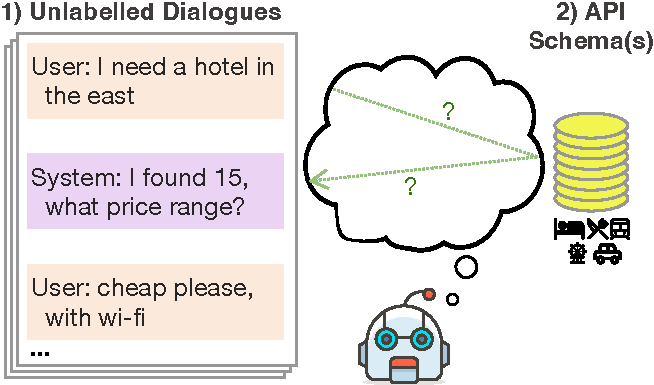
\includegraphics[width=\columnwidth]{imgs/fig_1_problem_v3.pdf}
    \caption{An overview of our unsupervised dialogue problem. We assume 1) unlabelled goal-oriented dialogues between a user and agent and 2) a well-defined schema $\schema$ with APIs suitable for fulfilling goals. We infer the unseen interactions between the agent and API, and use this to produce an end-to-end dialogue agent.}
    \label{fig:problem}
    % \vspace{-5mm}
\end{figure}
% The takeaway I want a reader to have is that while LLMs are great, the structured approach is worth pursuing and can be done.

Recent work has shown that LLMs can accomplish a broad set of useful tasks without any structured labels for a task \cite{brown_language_2020}. These include `zero-shot' approaches to task-oriented dialogue sub-tasks such as Dialogue State Tracking (DST) \cite{hu_-context_2022, king-flanigan-2023-diverse, heck-etal-2023-chatgpt}, intent detection \cite{pan_preliminary_2023}, grounded response generation \cite{li2023guiding-fix-arxiv}, and even zero-shot end-to-end dialogue systems \cite{hudecek-dusek-2023-large}. 
Still, existing approaches generally do not perform well enough for real-world use, and none are able to make effective use of in-domain unlabelled dialogues.


\begin{comment}
The motivation for such a system is the following. If a dialogue task is of high value but there is no existing dialogue system performing the task, then there are likely human agents performing the task while interfacing with users, and these conversations could be recorded. Additionally, a software developer likely has access to or can write a natural language API description for the API system that is supporting the task.   
\end{comment}
We ask: can we use existing unlabelled dialogues (without any labels or API calls annotated) along with an API specification, to build a working dialogue agent, without needing an expert to annotate data?
This addresses a common real-world scenario. 
Many high value dialogue tasks are currently carried out by human agents, who interface a user with some software system. 
These conversations can be recorded and transcribed, and the API(s) supporting the agent typically have well-formed specifications.
However, annotating the API calls and system acts needed for aligning the two is time consuming and requires annotation expertise.
In lieu of this, `zero-shot' systems have been proposed, but these still require an expert to annotate a `formatting example' \cite{hu_-context_2022, king-flanigan-2023-diverse}, or a more detailed `policy skeleton' \cite{zhang-etal-2023-sgp}.
%Thus we focus on the question of whether unlabeled dialogues (dialogues without any labels or API calls annotated) can facilitate building a zero-shot task-oriented dialogue system.

\begin{comment}
    Old comments/notes, prior to Jeff edits:
    % Challenges specific to our problem
    %We propose a method for leveraging LLMs in an unsupervised setting: in which plenty of available human-human dialogues in natural language are available, as well as a defined API schema, but there are no annotations aligning the two. 
    %In doing so we aim to answer (1) whether a system developer can implement a conversational AI from unlabelled dialogue without any assistance from an expert annotator and (2) whether the modular approach to end-to-end dialogue can still be successful in the absence of labelled module outputs. 
    % \bdk{Not sure our baselines suggest we have directly answered (2), may be worth discussing if this is a point we'd like to make.}
    % Our contributions
    %\bdk{Our Contributions section, this part is in a scratch-pad state relative to the rest.}
\end{comment}
We instead propose the following setting: we assume an API schema definition $\schema$, and plenty of available human-human dialogues in natural language, but no annotations on these dialogues (\autoref{fig:problem}). To the best of our knowledge, we are the first to consider this setting.
We demonstrate that one can develop a conversational agent for the API schema in this setting without any assistance from an expert annotator.  
Our contributions are as follows:
\begin{itemize}
    % Goal: take as much credit for proposing this setup as we reasonbly can, in context of existing work
    %\item To our knowledge, we are the first to construct a \textbf{performant} end-to-end task oriented dialogue agent solely from unlabelled dialogues and an API definition, without any turn-level labels. \bdk{I don't like `performant' here, but we'll need some way to account for a couple minor works}
    % What sets us apart from prior works? Using LLMs effectively 
    \item We construct an end-to-end task-oriented dialogue agent with an LLM solely from unlabelled dialogues and an API definition, without any turn-level labels or supervision from de-lexicalized utterances.
    % What sets us apart from prior works? Using LLMs effectively 
    \item We accomplish this by inferring all the pseudo-labels necessary (API calls, system actions) to train a traditional end-to-end dialogue system from unlabelled dialogues, using prompts which are automatically generated from the API schema.
    \item We propose a noisy-channel `code-to-text' re-ranking method, which is instrumental to our pseudo-label quality and final system.
    % \item Our hard Expectation-Maximization \cite{dempster_maximum_1977_fixed} approach leverages in-context learning with large language models by using our own predictions as future exemplars, and finally as data for a fine-tuned model.
    \item We devise a novel Hard-EM \cite{dempster_maximum_1977_fixed}\jmf{fix for camera-ready} approach which uses predictions as in-context examples for the LLM, and additionally as data for iteratively fine-tuning a final model.
    % Emphasize an important part of our techinical approach others could adapt
    
    %\item \jmf{We develop a general method for inferring API calls}
    %\item \jmf{We repurposed Multi-woz for evaluation for this setting}
    %\item \jmf{We are treating multi-woz as API calls, so we can apply code generation methods for inferring API calls to it}
\end{itemize}

\section{Preliminaries}

A task-oriented dialogue consists of turns of utterances between a user and an agent which interfaces the user with a programmable system or API to accomplish a task. Typically the system response utterance follows the user's utterance.
We denote $u_t$ as the user's utterance at turn $t$, and $r_t$ as the system's response. 
We assume the APIs supported by the system are defined in a schema $\schema$, which gives names and descriptions for all arguments supported in each API, as well as the possible values any categorical arguments may take \cite{rastogi_towards_2020}. 
This is analogous to standardized formats for API documentation, many of which could be easily converted to a schema definition.

Task-oriented systems require some method for interacting with the APIs in $\schema$. 
Modular approaches use a Dialogue State Tracking (DST) module, which predicts a belief state $b_t$\jmf{should we call this API call(s) instead?}: a collection of arguments to API call(s) needed to satisfy the user's goal. 
A belief state is commonly represented with a set of slot-value pairs:
$$
b_t = \{(s_1, v_1), (s_2, v_2), ... (s_n, v_n)\}
$$
For example, if a user says `I'm looking for a restaurant south of town', a DST system might produce the belief state \{(restaurant-area, south)\}, which can be used to query a restaurant API. We assume zero labeled belief states and infer them from unlabelled dialogues using the space of possible states supported by the schema definition $\schema$.

We also make use of system dialogue acts to structure our agent's communicative intents with a policy module. 
Given a dialogue state and context for a turn $t$, the policy predicts set of dialogue acts to be communicated in the system response $r_t$. 
For instance, the policy might determine that we should ask the user to narrow their search to a price range: $A_t = \{\text{Request(restaurant-area=?)}\}$.
An appropriate system response might be: ``Sure, are you looking for a particular price range?"
Like belief states, we assume zero supervised examples of $A_t$ and infer them from unlabelled dialogues. 

\section{Method Overview}
\label{sec:methods-overview}
\begin{figure*}
    \centering
    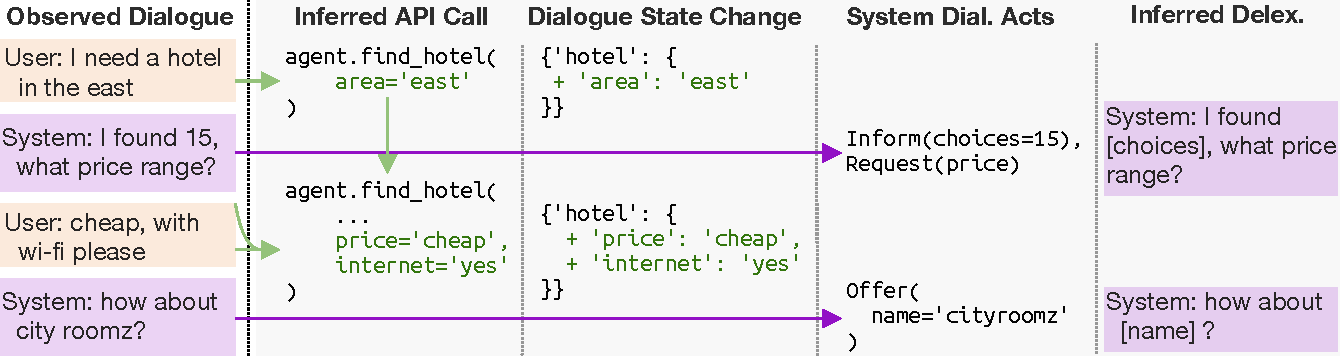
\includegraphics[width=\textwidth]{imgs/figure_2_latents_v4.pdf}
    \caption{An overview of the latent variables annotated in our unsupervised labeling process which are used to train the dialogue model. Our \dstcolor{DST Module} (\autoref{sec:methods-dst}) infers the API call(s) with arguments at each turn, from which we can derive the dialogue state change. Our \datcolor{DAT or Act Tagging module} (\autoref{sec:methods-tagging}) predicts the dialogue acts communicated in the observed system response, which can be used to infer de-lexicalized responses for training a response generator.\jmf{We could remove the dialogue state change column, and in the text say that we convert an API call to a dialogue state for evaluation (and give an example)} \bdk{Switched positions so its API -> dialogue state. Left it in as a column to make sure people who know MWoZ can very quickly understand the API call/state mapping}}
    \label{fig:latents-overview}
\end{figure*}
% Goal: it should be clear to reader what the modules we build are (in the entire system), their basic purpose, and which ones we have supervised data for/don't.
% Things that may not matter yet: our online in-context learning approach, text-to-code, exact inputs/outputs, iterative repeating of EM, etc.
% We construct `modularly end-to-end' dialogue system from unlabelled dialogues using expectation-maximization (EM) \cite{dempster_maximum_1977_fixed}.
We treat the turn-level labels needed for training an end-to-end dialogue system as a latent variables, and infer them from unlabelled dialogues.
We assume only the fully-lexicalized sequence of user and system utterances $u_1, r_1, ... u_T, r_T$, and the schema $\schema$ defining the system's capabilities, which defines the space of valid dialogue state and act labels. 
Importantly, our prompts are automatically generated from the API schema.

In \autoref{sec:methods-offline-label}, we outline our noisy-channel prompting method for inferring the turn-level labels necessary for training our dialogue agent. We give an overview of the latent variables we infer in \autoref{fig:latents-overview}. We assume we cannot query the APIs or observe results while labeling dialogues offline, as the obtained API results may have changed.
In \autoref{sec:methods-online-system}, we train a complete dialogue agent by fine-tuning on prompts derived from our inferred pseudo-labels.


% \jmf{Connect to unsupervised tool use}
\section{Inferring Latents via Noisy Channel}
%\subsection{Initial Labeling via Text-to-Code Prompting}
\label{sec:methods-offline-label}
% key-words: text-to-code, in-context learning, code LLMs
% Goal: first point someone should understand is what labels we predict and how. Secondary items to mention: in-context learning with iteratively loaded example pool, interchange-ability of kwargs in the prompt, anything else, that our prompt is not hand-crafted to a given schema.

% Module name/purpose
% How: prompt type, inputs, outputs.
% Repeat for other module
In this section, we present our method for inferring latent annotations for the dialogue states $b_1...b_T$\jmf{API calls?} and dialogue acts $A_1...A_T$ for each dialogue turn $t$ given only the unlabelled user and system utterances $(u_1, r_1, u_2, r_2, ... u_T, r_T)$.
% Given only unlabelled user and system turns for each dialogue $(u_1, r_1, u_2, r_2, ... u_T, r_T)$, we infer latent annotations for the dialogue states $b_1...b_T$ and dialogue acts $A_1...A_T$ for each turn $t$, overviewed in \autoref{fig:latents-overview}. 
To do this, we devise a noisy-channel prompting approach for DST and dialogue act tagging (DAT) using StarCoder \cite{li2023starcoder}, a code-based LLM.
First, we use a text-to-code prompt to infer the API call(s) made by the system in each dialogue, and build the dialogue state from inferred API call arguments (\autoref{sec:methods-dst}).
We use a similar text-to-code prompt to infer the latent act(s) communicated in each agent response, so that we can reverse-engineer an agent's policy (\autoref{sec:methods-tagging}).
For both tasks, we find much better performance when re-ranking latent predictions according to a noisy-channel model, in which we condition the observed utterance on a predicted latent in a code-to-text prompt (\autoref{sec:methods-nc-prompting}).
Finally, we leverage the in-context learning ability of LLMs by re-using our predictions as exemplars (\autoref{sec:methods-retriever}).
Given these initial pseudo-labels, we iteratively improve their quality using Hard-EM \cite{dempster_maximum_1977_fixed} (\autoref{sec:methods-re-labeling}).

\begin{comment}
\bdk{moving this figure to the Appendix as two full-page figures}
\begin{figure*}[h]
    \centering
    \begin{subfigure}[b]{0.48\textwidth}
        \centering
        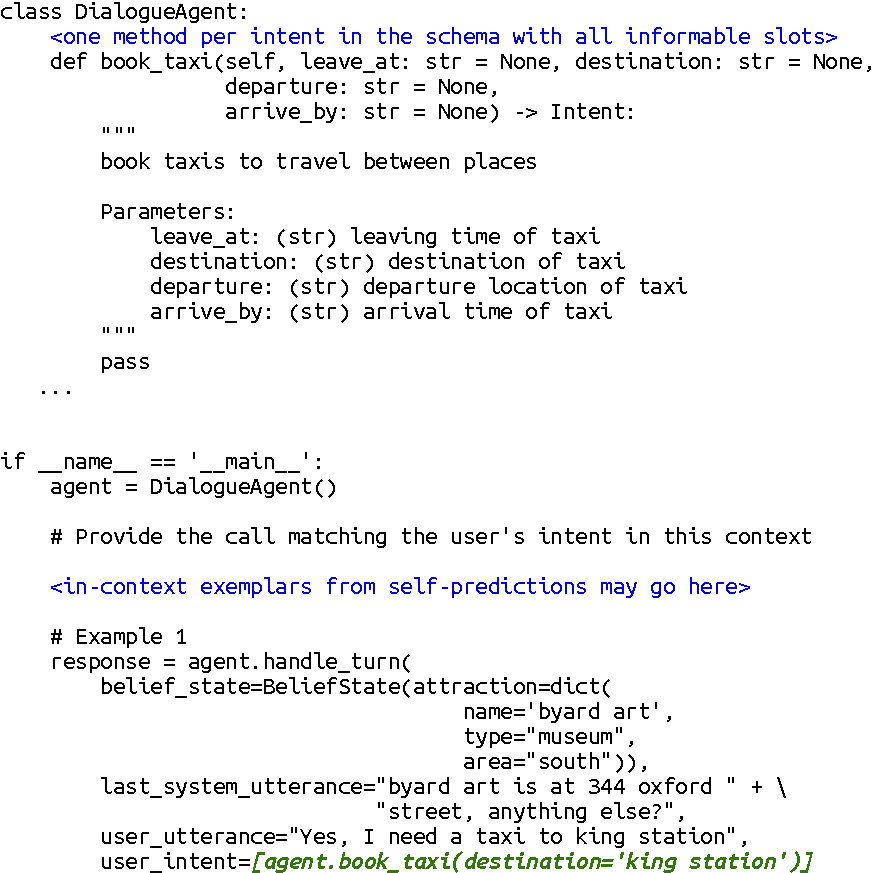
\includegraphics[width=\textwidth]{imgs/direct_dst_prompt_v5.pdf} % First image file
        \caption{Our `direct' DST prompt with italicized \dstcolor{\textit{\textbf{completion}}}}
        \label{fig:direct-dst-prompt}
    \end{subfigure}
    \hfill
    \begin{subfigure}[b]{0.48\textwidth}
        \centering
        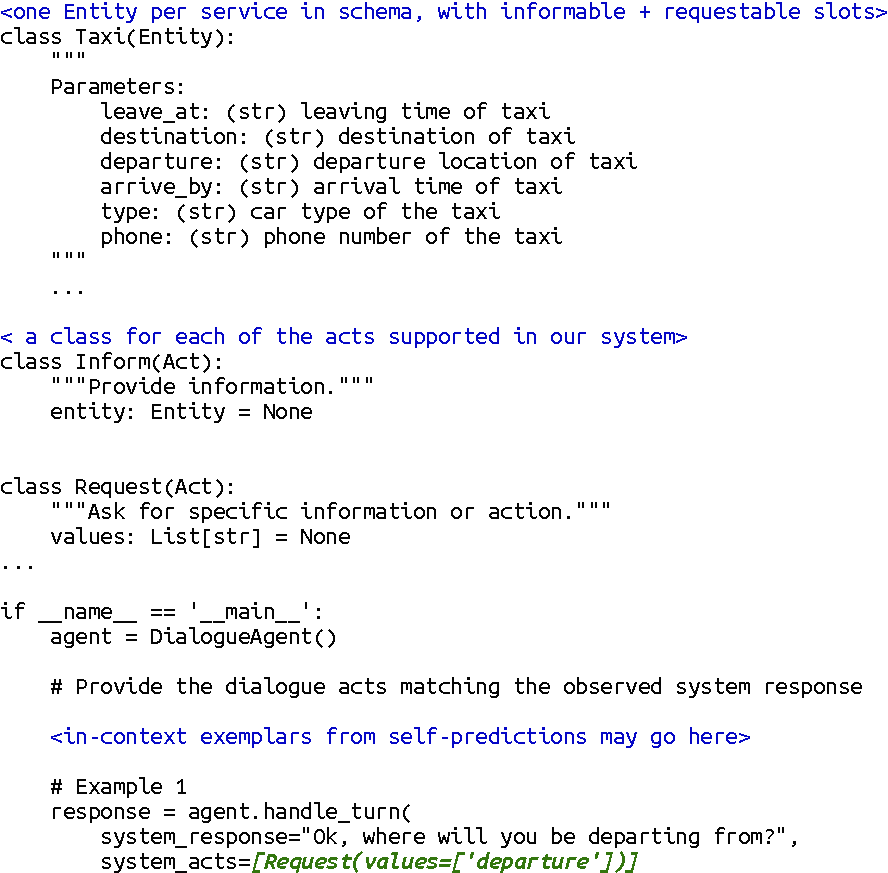
\includegraphics[width=\textwidth]{imgs/direct_dat_prompt_v3.pdf} % Second image file
        \caption{Our `direct' act tagging prompt, with italicized \dstcolor{\textit{\textbf{completion}}}}
        \label{fig:direct-act-tag-prompt}
    \end{subfigure}
    \caption{Abridged prompt and completion examples from our in-context learning approach to initial labelling for DST and DAT (Act Tagging), best viewed in color. Key-word arguments are used to include variables from the turn context and to prefix the completion}
    \label{fig:direct-prompt-examples}
\end{figure*}
\end{comment}

\subsection{Inferring API Calls and Dialogue State}
\label{sec:methods-dst}

We prompt the LLM with a text-to-code prompt for inferring the latent dialogue state as an API call.
\autoref{fig:direct-dst-prompt}  in \autoref{app:prompt-examples} gives an example of our prompt.
We generate a prompt enumerating the intents available in the schema $\schema$ as APIs callable by our agent.
Following \citet{hu_-context_2022}, we predict the appropriate function call conditioned on the prior system response $r_{t-1}$, the current user utterance $u_t$, and the previous belief state prediction $\hat{b}_{t-1}$. 
We then extract a dialogue state \textit{change} $\Delta \hat{b}_t$ from the arguments to the call, and compute the next dialogue state as $\hat{b}_t = \Delta \hat{b}_t + \hat{b}_{t-1}$.
While used offline here, this DST method is causal with respect to dialogue inputs and is the same as our method in online inference.

\subsection{Inferring System Acts} 
\label{sec:methods-tagging}
For inferring system acts, we use a similar text-to-code prompt for predicting the set of dialogue acts $A_t$ communicated in a given system response $r_t$.
See \autoref{fig:direct-act-tag-prompt} in \autoref{app:prompt-examples} for an example of our prompt.
We define each act our system could take in the prompt instructions.
For input from each turn, we find best performance when conditioning only on the response to tag, $r_t$.
For our set of supported acts, we use a subset of the universal dialogue acts proposed in \citet{paul19b_interspeech}, where some acts such as ``Inform'' or ``Offer'' may use slots defined in $\schema$.
For example, an agent choosing to offer to book a user at a hotel named `acorn guest house' might be represented as Offer(hotel\_name=`acorn guest house'). 
See \autoref{app:dialogue_acts} for our complete dialogue act set. 
Importantly, we use the schema definition $\schema$ and our act set to validate each act prediction, removing predicted keys which do not belong to $\schema$, or acts which are not in the set. For example, the `text' key is not valid for a `ThankYou' act, so a prediction of ``ThankYou(text=`thanks, have a good day')" would be normalized to only ``ThankYou()''.
Using the inferred system acts, we use a rule-based method to delexicalize the system responses for training the response generator (\autoref{fig:latents-overview}, right).
%These delexicalized responses are used when training a response generator.
\jmf{maybe also expand on this in the response generation section} \bdk{added under \autoref{sec:methods-online-system}, Response Generation.}

\subsection{Noisy Channel LLM Prompting}
\label{sec:methods-nc-prompting}

We find that a noisy channel prompting method \cite{min-etal-2022-noisy} significantly the quality of our inferred dialogue states and acts.
Here we describe noisy channel prompting using a simple example, and then describe its application to dialogue state tracking and system act tagging.

A typical prompt for machine reading comprehension might be:
% \vspace{-0.5mm}
\begin{Verbatim}[fontsize=\small]
    <Optional in-context examples (c)>
    Passage: <Passage (z)>
    Question: <Question (x)>
    Answer:
\end{Verbatim}
% \vspace{-0.5mm}

Given this prompt of the in-context examples $c$, passage $z$, question $x$, an answer $y$ completion is found with the language model by maximizing or sampling from $Pr(y|x,z,c)$.  We call this the \textbf{direct prompt}.

The \textbf{``noisy channel'' prompt} is:
% \vspace{-0.5mm}
\begin{Verbatim}[fontsize=\small]
    <Optional in-context examples (c)>
    Passage: <Passage (z)>
    Answer: <Answer (y)>
    Question: <Question (x)>
\end{Verbatim}
% \vspace{-0.5mm}
%where we score just the question, that is $Pr(x|y,z,c)$, following \citet{min-etal-2022-noisy}. To use the noisy channel LLM prompt, we first sample $k$ samples from the direct prompt, and then pick the best output answer $y$ according to the noisy channel prompt probability $Pr(x|y,z,c)$.
where the likelihood of the question now depends on the answer. 
To use the noisy channel LLM prompt, we first sample $k$ samples from the direct prompt, and then pick the best output answer $y$ according to the noisy channel prompt probability. 
One can choose to score the joint probability of the answer followed by the question, i.e. $Pr(x|y,z,c)Pr(y|z,c)$, or only the conditional $Pr(x|y,z,c)$, following \citet{min-etal-2022-noisy}.\footnote{In the latter case, the prior $Pr(y|z, c)$ is uniformly $\frac{1}{k}$ for the $k$ samples from the direct prompt.}

To apply this method to inferring dialogue states, we first sample a set of possible belief state changes using top-$p$ sampling \cite{holtzman_curious_2020} from the direct DST prompt, and then pick the best dialogue state according to the noisy channel prompt (see \autoref{fig:compare-direct-channel-dst}).  
We use an analogous procedure for inferring system acts.
For DST, we find scoring with the joint $Pr(x|y,z,c)Pr(y|z,c)$ to perform best, and scoring with the conditional $Pr(x|y,z,c)$ best for act tagging.

\begin{comment}
\begin{equation}
    \label{eq:direct_sample_dst}
    \C_{\Delta b_t} \topP P(\prompt(\Ek, \hat{b}_{t-1}, r_{t-1}, u_t))
\end{equation}

Where $\Ek$ is a set of $k$ in-context examples from a pool of our prior predictions, detailed below, and $\prompt$ combines arguments into our text-to-code prompt in the order they appear. 
We re-rank each candidate $\Delta b_t$ according to a code-to-text `channel' variant of the same prompt, where $p(y|x)$ is proportional to $p(x|y)p(y)$.
\end{comment}
\subsection{Retrieval-Augmented In-context Learning}
\label{sec:methods-retriever}
To leverage the in-context learning abilities of LLMs, we retrieve from a pool of examples from our predictions.
Because we assume no labeled examples, this pool starts with zero examples and is filled incrementally.
%We begin by initializing a pool of in-context examples $\Pool$ to retrieve from, starting with zero examples. 
%We then predict state and act labels for each turn and add it to the index $\Pool$ for use as an in-context example in the next iteration. 
We retrieve up to $k$ examples for in-context learning from this pool using an unsupervised dense retriever, with examples ranked by embedding cosine distance.\footnote{We use MPNet \cite{song_mpnet_2020}, available on Huggingface as \texttt{sentence-transformers/all-mpnet-base-v2}} 
We use $k=8$ and $k=6$ for DST, DAT respectively. 
For retriever inputs, we use $(\hat{b}_{t-1} \concat r_{t-1} \concat u_t)$ and $(u_t \concat r_t)$ for DST and DAT respectively, where $\concat$ indicates concatenation.
Applied naively, this in-context learning approach can suffer a majority label bias \cite{pmlr-v139-zhao21c}. We adjust for biases introduced in the initially small example pool by 1) not using any in-context examples until we have a minimum of $n=32$ examples in the pool and 2) using our API schema $\schema$ to require at least $4$ distinct labels in each set of in-context examples.\footnote{We consider two dialogue state change labels to be distinct if they update different \textit{slots}, and two act labels to be distinct if they embody different acts or different slots}
Our algorithm for producing initial pseudo-labels is in \autoref{app:offline_algorithm}.
\begin{figure}
    \centering
    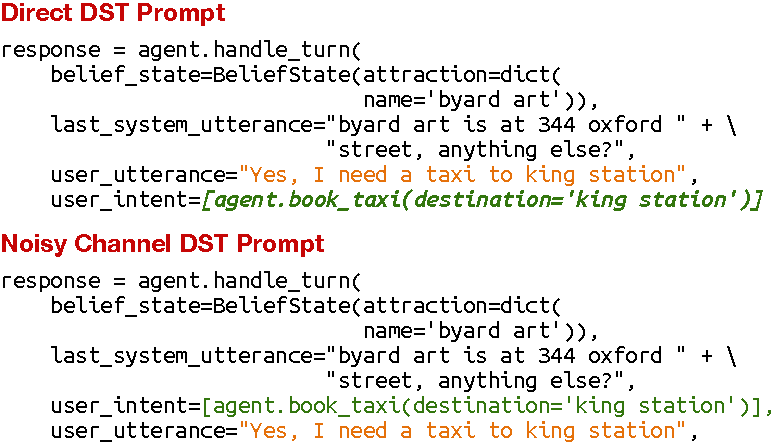
\includegraphics[width=\columnwidth]{imgs/fig_direct_vs_channel_dst_v2.pdf}
    \caption{Instances from our `direct' and `noisy channel' prompts for DST. Best viewed in color. After sampling a \dstcolor{\textbf{\textit{DST completion}}} from the `direct' prompt, we score it by the likelihood of the input \coloruser{user utterance} conditioned on it in the `noisy channel' prompt.} 
    \label{fig:compare-direct-channel-dst}
\end{figure}
\subsection{Refining the Labels with Hard-EM}
\label{sec:methods-re-labeling}

While the labels we produce in \autoref{sec:methods-dst}-\autoref{sec:methods-retriever} can be used directly for training an end-to-end dialogue system, we find their quality can be improved through expectation-maximization \cite{dempster_maximum_1977_fixed}.
For every dialogue turn in our dataset, our initial pseudo-labels provide the expected dialogue state and system dialogue acts according to our zero-shot system.
We then jointly fine-tune an LLM as a noisy-channel DST \& DAT system to maximize the likelihood of these expected labels.
We use smaller version of our prompted LLM, StarCoder 3B \cite{li2023starcoder}.

For each turn, we derive (prompt, completion) pairs for `direct' text-to-code and `channel' code-to-text DST and DAT modules, as defined in \autoref{sec:methods-offline-label}.
We then combine and shuffle these pairs into a single training set for joint fine-tuning.
For efficient training, we shorten our prompts by removing in-context examples as well as the function definitions used in the in-context learning setting. 
We find up-sampling the `channel' prompts so that there is a 2:1 ratio of `channel' to `direct' instances for training improves performance. 
% Complete training details are available in \autoref{app:training_details}.

After fine-tuning, the model can be used to produce improved pseudo-labels by re-labeling each dialogue, using the same noisy-channel inference methods. Following this, we can repeat the fine-tuning process.
This train and re-label process can be repeated for any number of iterations, though we find a single re-labeling is sufficient.

% %\subsection{Fine-tuning an end-to-end system}
\section{End-to-End System}
\label{sec:methods-online-system}
% % Main Goal: make clear how we train DST, Policy, Response Generation.

Following \cite{su-etal-2022-multi}, we utilize a multi-task fine-tuning method for training a single LLM as a complete dialogue system, consisting of a dialogue state tracker, policy, and response generator.

\paragraph{DST} For the DST sub-task, we again use both `direct' and `channel' (prompt, completion) pairs. 
This allows us to use the same noisy-channel inference method presented in \autoref{sec:methods-offline-label}.

% \subsection{Policy}
\paragraph{Policy} For the Policy sub-task, we use a text-to-code prompt where we simply condition on the $k$=5 most recent utterances in the dialogue history: $H_t = (u_{t-2}, r_{t-2}, u_{t-1}, r_{t-1}, u_{t})$. 
The completion is the current turn's system acts $A_t$, which will be used to ground the next response $r_t$. 
We do not use a noisy-channel variant for Policy, and greedily decode an act prediction at inference time:

$$
\hat{A}_t = \argmax{A_t \in \mathcal{V}^*}{P(\prompt(H_t)))}
$$

% "response_gen_simple": ["last_system_utterance", "user_utterance", "system_acts", "system_response"]

% \jmf{discuss delexicalization}
\paragraph{Response Generation} For Response Generation, we condition on the turn's observed system and user utterances $(r_{t-1}, u_t)$ and our policy's act prediction $\hat{A}_{t})$. The completion is the observed system response $r_t$. We also do not use a noisy-channel variant for response generation, and greedily decode the response:
$$
\hat{r}_t = \argmax{A_t \in \mathcal{V}^*}{P(\prompt(r_{t-1}, u_t, A_t)))}
$$
Following prior works, we predict \textit{delexicalized} responses, where values for slots in the system response are replaced with placeholders for the slot name. 
For example, instead of generating ``The phone number for acorn guest house is 555-5309" directly, we would predict ``The phone number for the [hotel\_name] is [hotel\_phone]'', where values could be filled in.
Importantly, we never presume access to gold delexicalized responses.
Instead, we use our predicted acts, e.g. ``Inform(name=`acorn guest house', phone=`555-8309')'', to delexicalize the observed response for training.

% \bdk{may need to collapse sub-sections to paragraphs, since this part isnt RG specific}
\paragraph{End-to-end Training} 
For each turn, we derive (prompt, completion) pairs for `direct' and `channel' DST, 
and direct Policy, and Response Generation prompts.
We then combine and shuffle these pairs into a single training set for joint fine-tuning.
For efficient training, we shorten our prompts by removing in-context examples as well as the function definitions used in the in-context learning setting. 
We find up-sampling the `channel' prompts so that there is a 2:1 ratio of `channel' to `direct' instances for training improves performance. 
Finally, we fine-tune StarCoder 3B using cross-entropy loss and AdamW with default hyperparameters. 

\begin{table*}[h!]
\centering
\begin{tabular}{lrrr|rrrr}
\textbf{Model} & \textbf{Schema?} & \textbf{Labels?} & \textbf{Dialogues?} & \textbf{Inform} & \textbf{Success} & \textbf{BLEU} & \textbf{Combined} \\
\hline
\multicolumn{8}{c}{\textbf{Supervised Results}} \\
\hline
%UBAR  & \cmark & \cmark & \cmark & - & - & - & - \\
%Soloist  & \cmark & \cmark & \cmark & - & - & - & - \\
%PPTOD  & \cmark & \cmark & \cmark & - & - & - & - \\
PPTOD \cite{su-etal-2022-multi} & \cmark & \cmark & \cmark & 82.6 & 72.2 & 18.2 & 95.6 \\
DiactTOD \cite{wu-etal-2023-diacttod} & \cmark & \cmark & \cmark & 89.5 & 84.2 & 17.5 & 104.4 \\
Our (supervised) & \cmark & \cmark & \cmark & 67.9 & 61.7 & 14.6 & 79.4 \\ 
%\devresult{Ours (supervised)} & \cmark & \cmark & \cmark & 62 & 55 & 11.9 & 70.4 \\

\hline
\multicolumn{8}{c}{\textbf{Zero-Shot with Formatting Example(s)}} \\
\hline
SGP-TOD-GPT3.5 \cite{zhang-etal-2023-sgp} & \cmark & Few (\ddag) & \xmark & 82.0 & 72.5 & 9.22 & 86.5 \\
\hline
\multicolumn{8}{c}{\textbf{Fully Unsupervised Results}} \\
\hline
% GPT 3.5 Turbo Baseline: https://wandb.ai/kingb12/llmbot/runs/urvyaats
%GPT 3.5 Turbo (ours delex) \cite{hudecek-dusek-2023-large} & \cmark & \xmark & \xmark & 44.8 & 31.2 & 3.31 & 41.31 \\
\multicolumn{8}{l}{\textit{\textbf{Sees gold delexicalized conversation history}}} \\
LLaMa\textsuperscript{\textdagger} & \cmark & \xmark & \xmark & - & 4 & 1.61 & - \\
GPT 3.5 Turbo\textsuperscript{\dag} & \cmark & \xmark & \xmark & 44.8 & 31.2 & 3.3 & 41.3 \\
\hdashline
\multicolumn{8}{l}{\textit{\textbf{Sees only fully-lexicalized dialogues}}} \\
GPT 3.5 Turbo ($-$ gold delex.) & \cmark & \xmark & \xmark & 40.7 & 26.7 & 3.7 & 37.4 \\
%GPT 3.5 Turbo (no delex) \cite{hudecek-dusek-2023-large} & \cmark & \xmark & \xmark & 40.7 & 26.7 & 3.68 & 37.38 \\
% Ours (no EM) == zero-shot: https://wandb.ai/kingb12/tod_zero/runs/rcjwoazq
Ours (StarCoder 15B - no EM) & \cmark & \xmark & \xmark & 50.0 & 19.6 & 3.2 & 38 \\
 %\devresult{Ours (ICL - StarCoder 15B)} & \cmark & \xmark & \cmark & 46 & 34 & 9.5 & 49.5 \\
% Ours (final) == 2-step EM: https://wandb.ai/kingb12/tod_zero/runs/zs0sv55o?nw=nwuserkingb12
Ours (StarCoder 3B - w/ EM) & \cmark & \xmark & \cmark & \textbf{78.1} & \textbf{68.3} & \textbf{13.6} & \textbf{86.8} \\
\hline
\end{tabular}
% \vspace{-2mm}
\caption{Unsupervised end-to-end results in MultiWOZ 2.2. (\dag) indicates models from \citet{hudecek-dusek-2023-large}. Results for LLaMa are from \citet{hudecek-dusek-2023-large}, which does not report the Inform rate. 
(\ddag) SGP-TOD uses a prompt with both a formatting example and a ``Policy Skeleton'', which contains an additional 10-20 hand-crafted instances of the correct system acts and response for an input user utterance or returned DB result. For fairer comparison in our fully unsupervised setting, we re-run the GPT 3.5 baseline without the supervision of de-lexicalized responses provided in the conversation history ($-$ gold delex.). Despite far fewer parameters, we find substantial improvements in our methods which leverage unlabelled dialogues}
\label{tab:main-results}
\end{table*}


\section{Experiments}

We conduct unsupervised end-to-end dialogue (E2E) and dialogue state tracking (DST) experiments on the MultiWOZ 2.2 dataset \cite{zang_multiwoz_2020, budzianowski2018large}, containing over ten thousand multi-domain task-oriented dialogues crowd-sourced in a wizard-of-oz setup. We use the fully lexicalized, unlabelled dialogues from the training set to build our system, and evaluate on the test set.
First, we demonstrate the value of our approach in an end-to-end dialogue evaluation, following prior works on task-oriented dialogue (\autoref{sec:expts-e2e}). 
Second, we conduct a dialogue state tracking evaluation to more carefully evaluate the quality of our pseudo-annotations (\autoref{sec:expts-dst}).
%\footnote{We do not conduct a similar analysis for Act Tagging since our universal act set derived from \citet{paul19b_interspeech} is not directly comparable to the domain-specific acts annotated in the MultiWOZ dataset}

\subsection{End-to-End (E2E) Experiments}
\label{sec:expts-e2e}

In E2E experiments, we use our complete system to both predict API call arguments and generate a next system response in natural language. 
We evaluate our generated responses with Inform rate, Success rate, and BLEU, as well as a Combined score of $0.5(\text{Inform} + \text{Success}) + BLEU$, following prior works. We provide details on these metrics in \autoref{app:metric_details}.

We compare our approach to the previous state-of-the-art unsupervised methods, a GPT-3.5 zero-shot baseline \cite{hudecek-dusek-2023-large}, and SGP-TOD \cite{zhang-etal-2023-sgp}. 
Where possible, we report results for both the original approach and modifications required to fit our fully unsupervised setting.
For reference, we also run our own method in the fully-supervised setting. 
We train a model using the procedure in \autoref{sec:methods-online-system} using the annotations sourced from crowd-workers in the MultiWOZ 2.2 corpus \cite{budzianowski2018large, zang_multiwoz_2020}, rather than the pseudo-labels predicted in \autoref{sec:methods-offline-label}.
We also compare with existing supervised approaches as a reference point. 
We include DiactTOD \cite{wu-etal-2023-diacttod}, which to our knowledge is the supervised state-of-the-art, and PPTOD \cite{su-etal-2022-multi}, which uses a multi-task fine-tuning approach similar to our own in \autoref{sec:methods-online-system}, for T5 encoder-decoder models \cite{raffel_exploring_2020}.

\subsection{DST Experiments}
\label{sec:expts-dst}

We conduct multi-domain DST experiments on the MultiWOZ Dataset in order to evaluate the quality of our pseudo-annotations. We use our DST Module to predict and evaluate only latent dialogue states, which collect the arguments required for unseen API calls.

Following prior works, we evaluate DST performance with joint-goal accuracy (JGA), or whether a given dialogue state is completely accurate. More details are available in \autoref{app:metric_details}.

We compare to our ChatGPT 3.5 Turbo baseline \cite{hudecek-dusek-2023-large}, as well as prior zero-shot DST methods.
These include IC-DST \cite{hu_-context_2022}, which re-frames DST as text-to-SQL, and RefPyDST which re-frames DST as text-to-python \cite{king-flanigan-2023-diverse}. By default, both of these works use OpenAI Codex \cite{chen_evaluating_2021}, and we apply their prompting approaches to StarCoder 15B for clearer comparison. 

\begin{table}[]
    \centering
    \resizebox{\columnwidth}{!}{
    \begin{tabular}{l|r}
        \hline
         \multicolumn{2}{c}{\textbf{With One Formatting Example}} \\
         \hline
         IC-DST (StarCoder 15B) & 24.58 \\
         RefPyDST (StarCoder 15B) & 17.17 \\
         IC-DST (Codex) & 35.02 \\
         RefPyDST (Codex) & 40.88 \\
         \hline
         \multicolumn{2}{c}{\textbf{Fully Unsupervised}} \\
         \hline
         IC-DST (StarCoder 15B) & 15.66 \\
         RefPyDST (StarCoder 15B) & 13.88 \\
         GPT 3.5 Turbo \cite{hudecek-dusek-2023-large} &  13.05 \\
         Ours (StarCoder 15B $\rightarrow$ 3B) & \textbf{39.70} \\ 
         % IC-DST Codex \cite{hu_-context_2022} & 175B & tbd \\ 
         % RefPyDST Codex \cite{king-flanigan-2023-diverse} & 175B & tbd \\
    \end{tabular}
    }
    % \vspace{-2mm}
    \caption{Joint Goal Accuracy (JGA) of our method's dialogue state predictions and zero-shot baselines}
    % \vspace{-4mm}
    \label{tab:zero-shot-multi}
\end{table}

\section{Results}
\label{sec:results}
\paragraph{E2E Performance} 
We present E2E results for our unsupervised dialogue agent in \autoref{tab:main-results}. 
We find that our method achieves state-of-the-art performance in our fully unsupervised setting, more than doubling the Success Rate and Combined score of the GPT 3.5 Turbo baseline of \citet{hudecek-dusek-2023-large}.
When we remove the supervision of delexicalization for fairer comparison ($-$ gold delex.), we find even greater improvement across all end-to-end metrics.
As discussed in \autoref{sec:related-work}, SGP-TOD uses both a supervised formatting example and a `Policy Skeleton', containing additional supervision for Policy and Response Generation.
With no implementation publicly available, we were unable to run a modified version of their experiments without this supervision for fair comparison. 
Despite a less-supervised setting, our method is able to perform comparably, even slightly out-performing SGP-TOD in Combined score.
% What to emphasize here will be pretty result-dependent, but options include low parameter count, performance relative to our supervised approach, performance relative to other supervised approaches.
Remarkably, our unsupervised EM approach also outperforms the supervised variant of our model due to improvements in Inform and Success rate, suggesting the Dialogue acts we infer are of high quality. 
% This may indicate noise in the system act labels provided with MultiWOZ, as they are annotated by crowd-workers \cite{budzianowski2018large}. 
% PPTOD \& DiactTOD may be robust to this noise because they pre-train on a policy across multiple dialogue datasets.
\paragraph{DST Performance} Our DST results are shown in \autoref{tab:zero-shot-multi}. Where possible, we distinguish between `zero-shot' results which include a hand-engineered formatting example, and the same method applied without the formatting example.\footnote{Due to the deprecation of OpenAI Codex, we were unable to run experiments for IC-DST or RefPyDST without a formatting example on the original Codex model}
We find that our method significantly outperforms our GPT 3.5 Turbo baseline by 26\% joint goal accuracy. 
Our approach performs nearly as well as the best method using OpenAI Codex with a supervised formatting example, using less than 10\% of the parameters at any time (175B vs. 15B). 
When applying the IC-DST and RefPyDST prompting methods to StarCoder, our method significantly outperforms both, with and without a formatting example.

\begin{comment}
When comparing to state-of-the-art zero-shot text-to-code approaches in \citet{hu_-context_2022, king-flanigan-2023-diverse}, we find our performs \maybe{comparably} despite our final inference model far fewer parameters.
One could conceivably use our approach with OpenAI Codex or a similarly large model and achieve further gains, but we choose to use an open model so that we can interrogate the pre-training data for contamination.   
\end{comment}


% Minus Noisy Channel Inference
% Minus EM
% Fine-tuning or ICL
% We handle both by just plotting across variants


\paragraph{Ablations} In \autoref{fig:success-v-steps}, we conduct an ablation to evaluate both the impact of our noisy channel modeling and the value of iterative re-labeling in our EM approach.
We compare our proposed system to one in which each module is replaced by only greedily sampling from its `direct' variant, at both labeling and end-to-end inference time. We plot our Combined end-to-end performance across iterations of EM, with `0' indicating our zero-shot system.
We find that EM improves our end-to-end performance in both our noisy-channel approach and greedy ablation, and that our noisy-channel inference methods are important to dialogue success, with a 30 and 33 point improvement over our greedy baseline with 1 and 2 EM steps, respectively. 
Ablations across Inform, Success, BLEU, and joint goal accuracy are in \autoref{app:additional-ablations}.

\begin{figure}
    \centering
    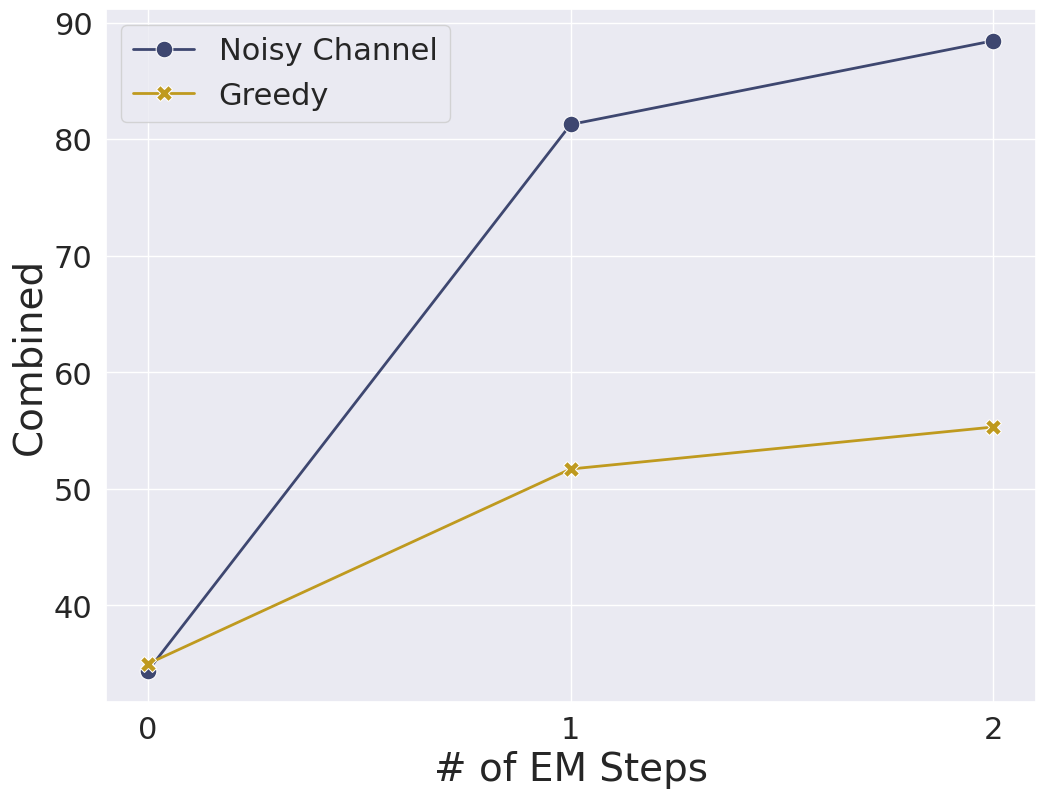
\includegraphics[width=\columnwidth]{imgs/step_plots_v3/combined_vs_steps.png}
    \caption{Combined score ($0.5(\text{Inform} + \text{Success}) + BLEU$) vs. the number of steps of expectation-maximization in our Noisy Channel method vs. a Greedy Ablation. `0' is zero-shot inference}
    \label{fig:success-v-steps}
\end{figure}
\begin{comment}
    \bdk{Removing this table in favor of a figure (graph)}
    \begin{table}[]
    \centering
    \resizebox{\columnwidth}{!}{
    \begin{tabular}{l|rrrr}
     & \textbf{Inform} & \textbf{Success} & \textbf{BLEU} & \textbf{Combined} \\
         \hline
         Greedy (zero-shot) & 32 & 4 & 2.66 & 20.66 \\ 
         Greedy (1-step) & 50.5 & 34.5 & 13.58 & 56.08 \\
         \hline
         Noisy Channel (zero-shot)  & 31 & 4.5 & 2.66 & 20.41 \\
         Noisy Channel (1-step) & 47 & 41 & \textbf{13.89} & 57.89 \\
         % Noisy Channel (2-step) & 28.1 & \textbf{49.5} & \textbf{44.5} & 12.88 & \textbf{59.88} \\
         
    \end{tabular}
    }
    \caption{Results on validation set\bdk{ablation results: until 1-step comes in for valid20p}}
    \label{tab:greedy_vs_nc}
\end{table}

\end{comment}

\section{Contamination Analysis}
\label{sec:contamination-analysis}

Evaluation of unsupervised methods, such as ours, that use LLMs has the potential issue of \textbf{task contamination}, where supervised examples are seen in pretraining data \cite{li_task_2024}.  Inclusion of supervised examples of the task in LLM pretraining data would render the model no longer unsupervised and the evaluation potentially biased: tasks for which the training data has been seen may have a higher performance than truly unsupervised tasks.

To address this issue, we quantify the presence of contamination in LLM pre-training data, and then estimate the potential impact on our results.
Fortunately, the StarCoder family of models that we use has the complete pre-training corpus publicly available for analysis.\footnote{\href{https://huggingface.co/datasets/bigcode/starcoderdata}{https://huggingface.co/datasets/bigcode/starcoderdata}}

\begin{comment}
In an ideal world, benchmarks of community interest would be completely and verifiably excluded from LLM pre-training.
Today's NLP ecosystem poses two obstacles to this.
First, many of the most capable LLMs are released without an open pre-training corpus.
Second, public use of benchmark data complicates exclusion: it is not sufficient to simply exclude the primary source of the benchmark.
To our knowledge, there are no suitably complex human-human task-oriented dialogue benchmarks that are guaranteed to be excluded from the pre-training of the most capable LLMs.

In light of this, we aim to first 
\end{comment}


\begin{table}[]
    \centering
    \begin{tabular}{l|r:rr}
         \textbf{Task} & \textbf{Turns} & \textbf{Correct} & \textbf{Authentic} \\
         \hline
         Act Tagging & 42 & 21 & 5 \\  
         DST & 42 & 36 & 19 \\  
    \end{tabular}
    \caption{Number of discovered contaminated turns per task, as well as the number which are correct or verified as being in the MultiWOZ dataset.}
    \label{tab:contamination}
\end{table}

%\paragraph{Contamination Findings}
We conduct an exhaustive search for supervised pairs of our dialogue subtasks in the StarCoder pretraining data using a semi-automated search with manual review.  Details of our search procedure are in \autoref{app:contamination_details}.  We find no complete dialogues with supervised labels.  We do find 42 turns labeled with act tagging, and 42 turns labeled with DST in the pre-training corpus, categorized in \autoref{tab:contamination}.\footnote{The average dialogue length in MultiWOZ is 13.9 turns. Put together, the set of contaminated turns would be roughly the length of 6 dialogues}
We consider a $(x, y)$ pair to be `Correct' if the state change/dialogue act $y$ is actually correct for the utterance $x$, and to be `Authentic' if the $(x,y)$ pair is found verbatim in the MultiWOZ corpus.\footnote{A `Correct' pair might arise from printing training data, and an incorrect pair from discussion of a failure case.}
Astonishingly, we find half of the found Act Tagging pairs are incorrect, and could possibly mislead a pre-trained model if the model learned from them.
We also find that less than half of the turns are authentic for either task, and find a number of them derive from Github issues discussing problems with dialogue simulators.

%\paragraph{Performance Comparison}
% Finally, we estimate the degree to which the contamination we discover could exaggerate expected performance of our method on an unseen schema $\schema$.
Additionally, we estimate the degree to which the contamination we discover could exaggerate expected performance of our method on an unseen schema, by using contaminated $(x, y)$ pairs as in-context examples.\footnote{Ideally, one would pre-train an identical StarCoder model on a corpus \textit{without} contamination, this is computationally impractical. Additionally, we are not aware of any available LLM that can be verified as not contaminated for this task.}

In \autoref{tab:contaminated_experiment}, we compare our zero-shot prompt, which receives no examples of any kind, with a `contaminated' variant which uses $k$=3 in-context examples derived from contamination in the pre-training corpus.
The `contaminated' model retrieves the most relevant contaminated fragments from a pool using the dense retrieval approach described in \autoref{sec:methods-retriever}. 
These are inserted as a triple-quoted string block, so that the prompt remains syntactically valid python.
By leaving contaminated examples in their original format, we test whether their inclusion elicits memorized knowledge rather than providing guidance on input/output formatting.
%\footnote{\citet{min-etal-2022-rethinking} find that GPT-3 performs almost as well when using \textit{random} labels in in-context examples, suggesting much of the value of comes from demonstrating the format}
Surprisingly, we find including this supervision via contaminated fragments \textit{hurts} performance, indicating that these examples do not provide meaningful supervision for our task.
Further, the substantial gains in our noisy-channel EM approach suggest our method is doing more than simply eliciting schema-specific knowledge memorized in pre-training.
 
\begin{table}[]
    \centering
     \resizebox{\columnwidth}{!}{
    \begin{tabular}{l|rrrr}
    \textbf{Method} & \textbf{Inform} & \textbf{Success} & \textbf{BLEU} & \textbf{Combined} \\
       \hline
       Ours (zero-shot) & \textbf{49.0} & \textbf{15.0} & 3.0 & \textbf{35.0} \\
       Ours (k=3 contam ex.) & 44.5 & 14.0 & \textbf{3.8} & 33.1 \\
       \hline
       Ours (Full EM) & \textbf{80.5} & \textbf{69.0} & \textbf{13.7} & \textbf{88.5} \\
    \end{tabular}
    }
    \caption{Performance comparison when we include contaminated in-context examples. We find \textit{including} this supervision hurts performance, and does not explain the strong performance of our noisy-channel EM approach}
    \label{tab:contaminated_experiment}
\end{table}

\section{Related Work}
\label{sec:related-work}

\paragraph{Zero-shot Dialogue} A few recent works have proposed zero-shot approaches to dialogue problems using LLMs. 
\citet{hu_-context_2022} and \cite{king-flanigan-2023-diverse} propose DST methods which prompt code based LLMs in a text-to-SQL or text-to-program format, respectively. 
These methods rely on prompts tailored to the schema and the use of a supervised `formatting' example, which requires annotation expertise. 
\citet{zhang-etal-2023-sgp} extends this approach to end-to-end task-oriented dialogue by adding a policy prompter for GPT 3.5. 
In addition to a formatting example, their policy prompt requires a hand-crafted `policy-skeleton' consisting of examples of the appropriate system act and reply in response to different user utterances or database results.
Our approach differs in that we require zero labeled examples of any kind. 
\citet{hudecek-dusek-2023-large} propose a zero-shot end-to-end method for prompting instruction-tuned LLMs like GPT 3.5.
However, this method presumes \textit{delexicalized} system responses $r_1 ... r_{t-1}$ in the conversation history as input, where entities are replaced with placeholders. 
Producing these inputs requires ground-truth annotations and gives a form of supervision about the entities and their attributes within a dialogue (see \autoref{tab:main-results} for a comparison for  GPT 3.5 Turbo with and without delex supervision).
In contrast, we only assume fully-lexicalized dialogues, which do not provide this supervision and require no human annotation.
We adapt the method of \citet{hudecek-dusek-2023-large} to use lexicalized dialogues as inputs, and use this approach as our baseline.
\citet{chung_instructtods_2023} propose an end-to-end method which prompts GPT-4 for interactions with a knowledge base before producing a response, however it generalizes poorly to the multi-domain setting.

\paragraph{Semi-supervised TOD} Some works propose semi-supervised approaches to end-to-end task-oriented dialogue. 
\citet{zhang_probabilistic_2020} propose an end-to-end sequence-to-sequence model where the dialogue state is a latent variable. 
\citet{liu_variational_2021} adapt this approach for use with pre-trained language models, fine-tuning GPT-2. 
While successful, these approaches require a non-trivial amount of supervised data.
Other semi-supervised works also evaluate their method in an unsupervised setting \cite{jin_explicit_2018, liu_unsupervised_2023}. 
However, these works also assume delexicalized training dialogues, which requires ground-truth annotation and gives a form a supervision to the model.

\paragraph{Noisy channel and re-ranking methods} 
A few previous works have utilized noisy channel methods for task-oriented dialogue or prompting methods. \citet{liu_pretraining_2021} pre-train a noisy channel for task-oriented dialogues as a sequence to sequence model, however their method requires significant labelled training data. \citet{min-etal-2022-noisy} propose noisy channel prompting for few-shot classification tasks, which inspires our generalization to the generative setting.

\section{Conclusion}

We present a novel approach for constructing an end-to-end task-oriented dialogue system by leveraging pre-trained language models to infer labels from unlabeled dialogues.

\section{Limitations}

Data contamination in LLM pre-training poses a hurdle for accurate benchmarking across NLP, and particularly for unsupervised methods.
In an idealized setting, there would be a suitably strong task-oriented dialogue benchmark that could be verified as not belonging to the pre-training corpus of each new and more capable LLM.
This is not the case for our setting or for many others, and warrants careful attention from the NLP community.
For our setting, we were able to properly define problematic contamination and search for it in our LLM's pre-training corpus, thanks to the open release of the pre-training data.
We found limited contamination and demonstrated that the contamination we found was not helpful in eliciting task knowledge that might have been memorized in pre-training. 
%However, our computational budget prevents us from conducting the ideal ablation, in which we pre-train another LLM without any contaminated data. 
%Strategies for quantifying and coping with contaminated data, as well as producing verifiably non-contaminated benchmarks are important directions for future work.
%We think it is valuable to seek and quantify benchmark contamination rather than assume it is not present or only use closed-data models which prevent such inquiry.

All experiments in this paper were conducted on pre-existing public dialogue corpora, collected explicitly for training task-oriented dialogue agents with the knowledge of all participants \cite{budzianowski2018large}. 
Our use of the StarCoder model also falls within the terms of it's Responsible AI License.
It is important that subsequent applications of our method also adhere to any fair-use policies governing collected dialogues or transcripts.

\bdk{Points to discuss: fair access and use of unlabelled dialogues}

% Entries for the entire Anthology, followed by custom entries
\bibliography{anthology,custom}

\appendix
\section{Prompt Examples}
\label{app:prompt-examples}
\autoref{fig:direct-prompt-examples} provides abridged instances of our direct prompts for DST and for Act Tagging. \autoref{fig:direct-dst-prompt} shows our prompt for inferring API call(s) or changes to the dialogue state from an unlabelled dialogue, as detailed in \autoref{sec:methods-dst}. Our prompts use python keyword arguments to provide the input variables for a given sub-task, and to prompt the LLM for the next variable of interest. Using the arbitrary ordering of keyword arguments in Python function calls, our `channel' prompts simply re-order the arguments in order to score the likelihood of the user's utterance given the predicted state change.
\autoref{fig:direct-act-tag-prompt} provides a similar abridged instance of our direct prompt for tagging dialogue acts in an unlabelled dialogue. Here, we simply condition on the observed system response $r_t$.

\begin{figure*}[h]
    \centering
    \begin{subfigure}[b]{0.49\textwidth}
        \centering
        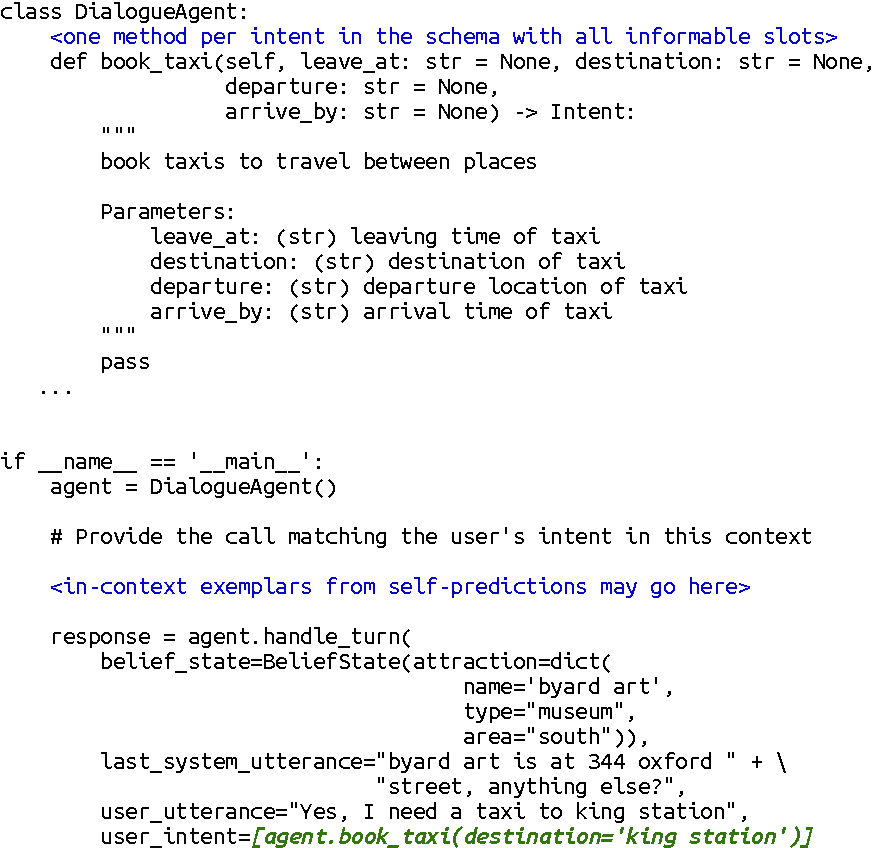
\includegraphics[width=\textwidth]{imgs/direct_dst_prompt_v6.pdf} % First image file
        \caption{Our `direct' DST prompt with italicized \dstcolor{\textit{\textbf{completion}}}}
        \label{fig:direct-dst-prompt}
    \end{subfigure}
    \hfill
    \begin{subfigure}[b]{0.49\textwidth}
        \centering
        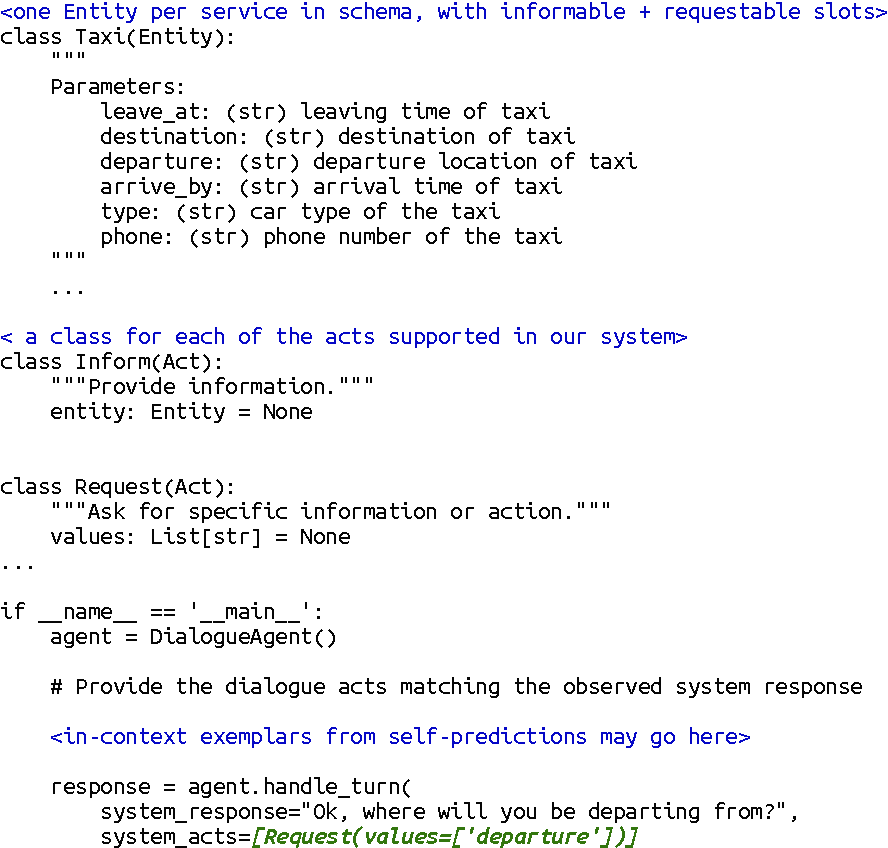
\includegraphics[width=\textwidth]{imgs/direct_dat_prompt_v4.pdf} % Second image file
        \caption{Our `direct' act tagging prompt, with italicized \dstcolor{\textit{\textbf{completion}}}}
        \label{fig:direct-act-tag-prompt}
    \end{subfigure}
    \caption{Abridged prompt and completion examples from our in-context learning approach to initial labelling for DST and DAT (Act Tagging), best viewed in color. Key-word arguments are used to include variables from the turn context and to prefix the completion}
    \label{fig:direct-prompt-examples}
\end{figure*}

%\section{Training Details}
%\label{app:training_details}
%Training details will go here.

\section{Metric Details}
\label{app:metric_details}
\paragraph{End-to-End (E2E) Dialogue Metrics}
We measure end-to-end dialogue performance using the Inform rate, Success rate, and BLEU, following prior works, using the automatic evaluation provided by \citet{nekvinda-dusek-2021-shades}.\footnote{\href{https://github.com/Tomiinek/MultiWOZ_Evaluation}{https://github.com/Tomiinek/MultiWOZ\_Evaluation}}

A dialogue is considered Informed if the most recently mentioned result for each domain meets the user's goal constraints, and is considered Successful if it is Informed and all values for requested slots are presented to the user. 
For example, if a user were to ask `Can you give me the phone number of a cheap hotel in the east part of town?', the dialogue would be Informed if we refer them to a hotel that is actually in the cheap price range and in the east, and Successful if we additionally provide the phone number, as requested. 
BLEU is computed against a single reference response, and the Combined score is $0.5(\text{Inform} + \text{Success}) + BLEU$.

\paragraph{Dialogue State Tracking Metrics} 
Following prior works, we evaluate DST performance with joint-goal accuracy (JGA): for a turn $x_t$, a dialogue state prediction $\hat{y}_t$ is considered correct only if all slot names and values match the gold annotation state $y_t$. We again use the evaluation provided in \citet{nekvinda-dusek-2021-shades}. Following their work, we accept fuzzy matches for non-categorical string values, such as the name of a restaurant or hotel, using the \texttt{fuzzywuzzy} library and a fuzz ratio of 0.95.\footnote{\href{https://pypi.org/project/fuzzywuzzy/}{https://pypi.org/project/fuzzywuzzy/}} 

\section{Dialogue Acts}
\label{app:dialogue_acts}

Following \citet{paul19b_interspeech}, we use a universal set of dialogue acts for managing our agents communicative intents. We omit some acts for simplicity and to reduce the context length required to enumerate them in a prompt. \autoref{tab:dialogue_acts} lists each act and a description. Since our dialogue set is not directly comparable to prior works, we do not directly evaluate act tagging or policy accuracy. Instead, acts serve only as an intermediate representation for planning responses in our end-to-end system.

\begin{table*}[]
    \centering
    %\resizebox{\textwidth}{!}{
    \begin{tabular}{l p{12cm}}
        \textbf{Act} & \textbf{Description (as used in our prompt)} \\
        \hline
         Inform(x=y) &  Provide information. \\
         Offer(x=y) &  System provides an offer or suggestion based on results. \\
         Confirm(x=y) &  Seek confirmation of something. \\
         Affirm(x=y) &  Express agreement or confirmation. \\
         Negate(x=y) & User or System denies or negates. \\
         NotifySuccess(x=y) & Notify of a successful action or result. \\
         NotifyFailure(x=y) & Notify of an error or failure. \\
         Acknowledge & Acknowledge. \\
         Goodbye & Goodbye. \\
         Greeting & Greeting. \\
         ThankYou & ThankYou. \\
         RequestAlternatives & Ask for other options, alternatives, or any additional user goals. \\
         Request(x=?) & Ask for specific information or action. \\
         
         & 
    \end{tabular}
   % }
    \caption{Dialogue acts supported by our system, adapted from the universal dialogue acts proposed in \citet{paul19b_interspeech}. ``x=y" indicates the act can take on arbitrary key-value arguments, and ``x=?" indicates the act takes on one or more unpaired arguments. We reduce the number of acts and lengths of descriptions relative to \citet{paul19b_interspeech} in order to fit within the LMs context length}
    \label{tab:dialogue_acts}
\end{table*}

\section{Offline Labeling Algorithm}
\label{app:offline_algorithm}

\textbf{Algorithm 1} gives our algorithm for pseudo-labeling of unlabelled dialogues.

\begin{algorithm*}
\label{alg:offline_label}
\begin{algorithmic}[1] % The number tells where the line numbering should start
\Procedure{InitialOfflineLabel}{$\D_{train}, \retriever$, $\LM$} % Procedure name and parameters
    \State $\Pool \gets \emptyset$ \Comment{Initialize example pool}
    \State $\mathcal{B} \gets []$ \Comment{Store predictions by dialogue id and turn index}
    \For{$t = 0$ \textbf{to} $\maxunderset{d \in \D_{train}}{|d|}$} \Comment{Loop by increasing turn index}
        \ForAll{$(d_{id}, u_t, r_{t-1}, r_t)$ \textbf{in} $\D_{train}$} \Comment{$d_{id}$ is dialogue ID}
            \State $\hat{b}_{t-1} \gets \mathcal{B}[d_{id}][t-1] \textbf{ or } \emptyset$ \Comment{Fetch $\hat{b}_{t-1}$ if known}
            \State $\hat{b}_t \gets \Call{OfflineDST}{\Pool, \retriever, \hat{b}_{t-1}, r_{t-1}, u_t}$
            \State $\hat{A}_t \gets \Call{OfflineActTag}{\Pool, \retriever, u_t, r_t}$
            \State $\Pool \gets \Pool \cup \{(r_{t-1}, u_t, r_t, \hat{b}_t, \hat{A}_t)\}$ \Comment{Add in-context example for future labeling}
        \EndFor
    \EndFor
\EndProcedure
\Procedure{OfflineDST}{$\Pool, \retriever, \hat{b}_{t-1}, r_{t-1}, u_t$}
    \State $\Ek \gets \retriever(\hat{b}_t \concat r_{t-1} \concat u_t, \Pool)$ \Comment{Retrieve up to $k$ in-context examples}
            \State $\C \gets \Delta b_t \topP P(\prompt(\Ek, \hat{b}_{t-1}, r_{t-1}, u_t))$ \Comment{Sample w/ `direct' prompt}
            \State $\Delta \hat{b}_t \gets \argmax{\Delta b_t \in \C}{P(u_t | \prompt(\Ek, \hat{b}_{t-1}, r_{t-1}, \Delta b_t)}$ \Comment{Re-rank w/ `channel' prompt}
            \State \Return $\hat{b}_{t-1} + \Delta \hat{b}_t$
\EndProcedure
\Procedure{OfflineActTag}{$\Pool, \retriever, u_t, r_t$}
    \State $\Ek \gets \retriever(u_t \concat r_t, \Pool)$ \Comment{Retrieve up to $k$ in-context examples}
            \State $\C \gets A_t  \topP (P(\prompt(\Ek, r_t)))$ \Comment{Sample w/ `direct' prompt}
            \State \Return $ \argmax{A_t\in \C}{P(\Ek, A_t, r_t)}$ \Comment{Re-rank w/ `channel' prompt}
\EndProcedure

\end{algorithmic}
\caption{Our algorithm for initial pseudo-labeling of unlabelled dialogues in $\D_{train}$}
\end{algorithm*}

\section{Further results across EM Steps}
\label{app:additional-ablations}

Here we expand on our ablations in \autoref{sec:results}, which evaluates our method with and without our proposed noisy-channel prompting across iterations of expectation-maximization (EM). In \autoref{fig:app-step-plots-grouped}, we break down the performance gains we observed in our `Combined' metric into Inform rate, Success rate, and BLEU, where $\text{Combined} = 0.5(Inform + Success) + BLEU$. `0' iterations of EM indicates our zero-shot prompting system, without any in-context examples or EM. We find that EM substantially improves performance in all cases, and particularly for our noisy-channel prompting approach. We find the noisy channel prompting approach improves performance on all metrics, with the most substantial gains over the greedy baseline in Inform and Success rates. 
This suggests that within our algorithm, noisy-channel inference may be particularly important when inferring the system's dialogue acts in order to reverse-engineer an accurate policy.

In \autoref{fig:app-jga-over-steps}, we analyze dialogue state tracking performance across iterations of EM using Joint Goal Accuracy (JGA). We find our noisy-channel prompting approach improves the accuracy of our dialogue state tracking predictions across iterations of EM when compared to a greedy, direct prompting approach.

\begin{figure*}
    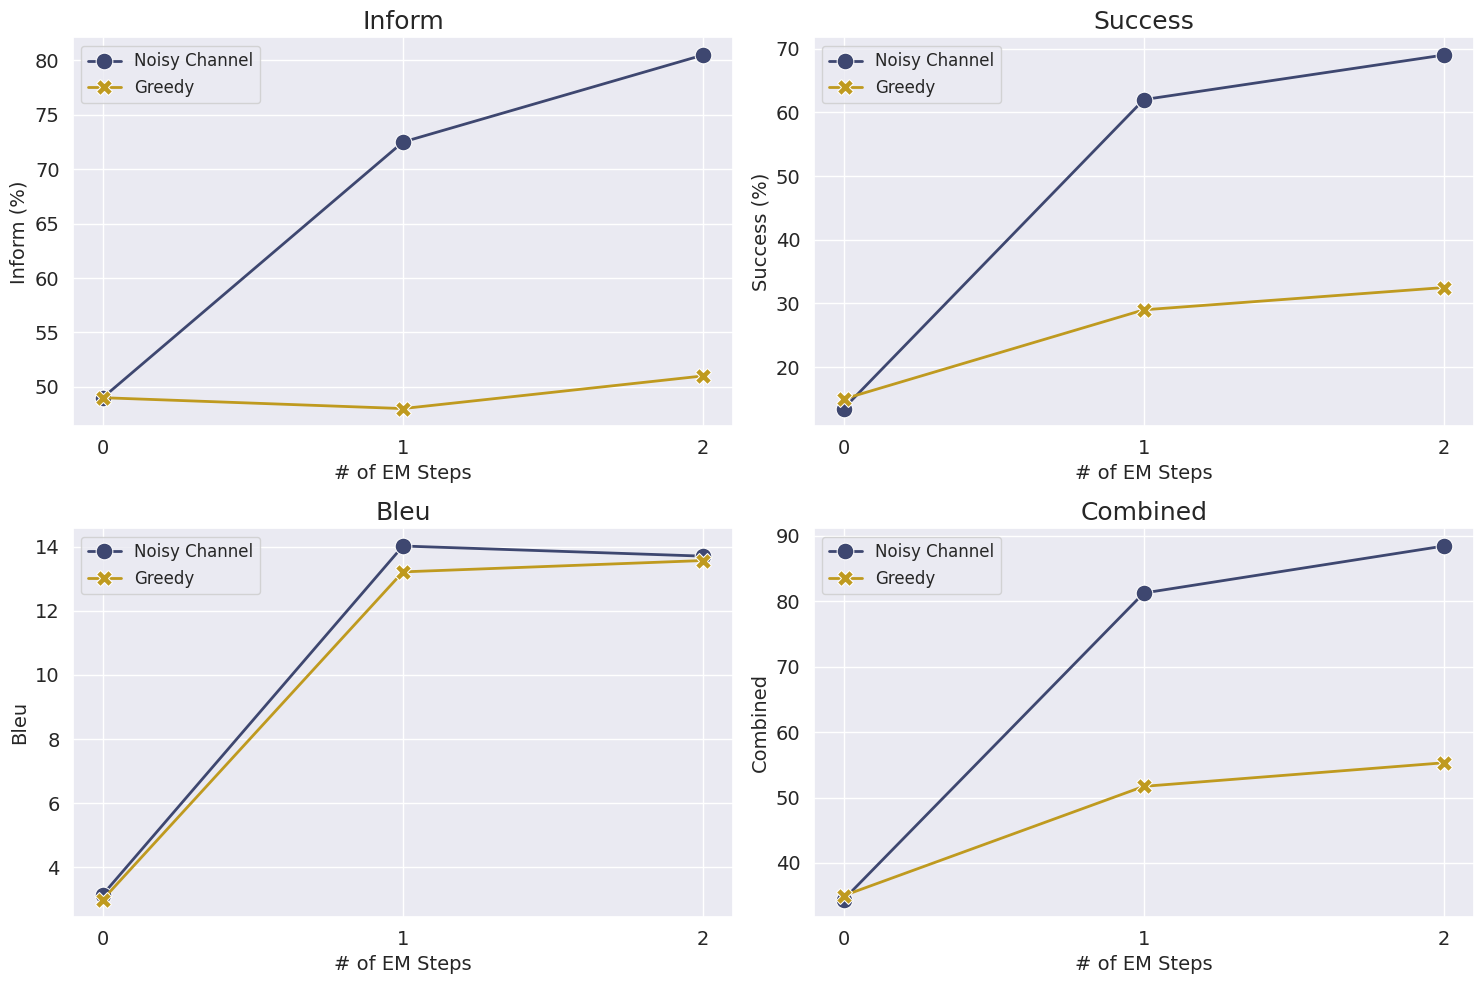
\includegraphics[width=\textwidth]{imgs/step_plots_v2/inform_success_bleu_combined_multi_plot.png}
    \caption{Breaking down $\text{Combined} = 0.5(\text{Inform} + \text{Success}) + BLEU$ into components Inform Rate, Success Rate, and BLEU across iterations of EM between our proposed noisy-channel approach and a greedy ablation, which omits noisy-channel prompting at inference time and when labeling dialogue states \& system acts in the expectation step. We find improvement across all components, and particularly our Inform and Success Rates}
    \label{fig:app-step-plots-grouped}
\end{figure*}

\begin{figure*}
    \centering
    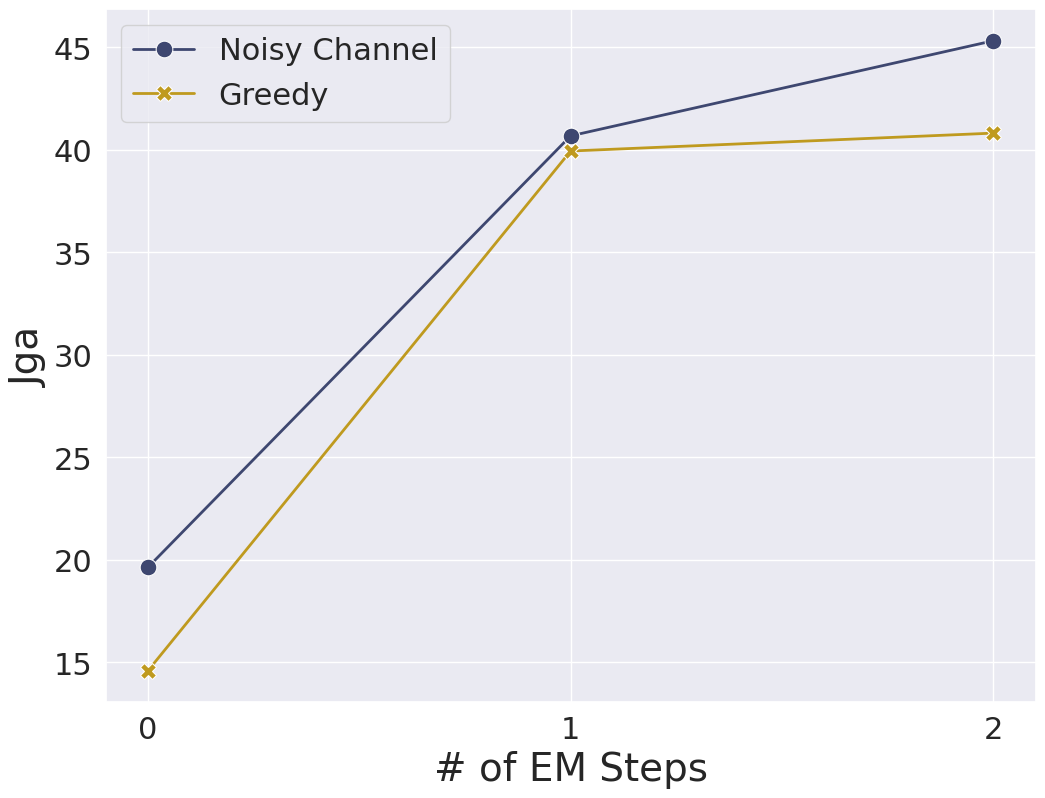
\includegraphics[width=0.5\textwidth]{imgs/step_plots_v3/jga_vs_steps.png}
    \caption{Joint Goal Accuracy (JGA) of our inferred API call(s)/Dialogue states across iterations of EM. We find improved dialogue state tracking performance when using our noisy-channel method at inference time and when labeling dialogue states offline in the expectation step for training, compared to a greedy direct prompting approach}
    \label{fig:app-jga-over-steps}
\end{figure*}



\section{Contamination Search \& Result Details}
\label{app:contamination_details}

\subsection{Procedure} 

We detail our method for finding instances of task contamination within the StarCoder pre-training set.
We are particularly interested in \textit{supervised pairs $(x, y)$} where $y$ belongs to our schema of interest $\schema$, for any of the dialogue sub-tasks used in our system. 
We devise a method for searching the complete pre-training corpus for contaminated $(x, y)$ pairs, where $x$ is an utterance we might observe from either the system or user, and $y$ is the latent dialogue state change or dialogue act supporting $\schema$. 
For each utterance $x$ from either the system or user, we collect all documents from the pre-training corpus which contain the complete utterance. 
We use the elastic search index provided for the StarCoder pre-training data, which accounts for differences in capitalization, punctuation, and interrupting white-space.\footnote{\href{https://github.com/bigcode-project/search/blob/main/index.py}{https://github.com/bigcode-project/search/blob/main/index.py}} 
Following this, we search matching documents for keywords from $y$ (e.g. slot names and values) to determine which of these documents may plausibly contain a supervised label and warrant manual review. 
For dialogue states, these are the slot names and values, discarding extremely generic keywords like `name'.
For act tags, these are the act names, slots, and values.
We then consider a document to need manual review if 40\% or more of the keywords are found in the 500 characters before or after a matching $x$ in a document.
Finally, we hand-check the remaining documents and extract contaminated $(x, y)$ pairs.


\subsection{Examples}
\autoref{tab:contamination-examples} contains examples of contamination discovered in our search process, and the type of document in which they were found. Notably, none of the examples found closely match our output formatting.

\begin{table*}[htbp]
    \centering
    %\resizebox{\textwidth}{!}{
    \begin{tabular}{>{\raggedright\arraybackslash}p{0.25\textwidth}|>{\raggedright\arraybackslash}p{0.25\textwidth}|r|r}
        \textbf{Contaminated Input} & \textbf{Contaminated Output} & \textbf{Sub-Task} & \textbf{Source}  \\ 
        \hline
         I need a restaurant to dine at in Cambridge on my upcoming trip . I need info about chiquito restaurant bar restaurant . & restaurant-inform<<<name===chiquito restaurant bar & DST & Jupyter Notebook \\
         \hline 
         i would like to book a 5 star , or closest to it , in the east part of town please . & "<SOB> hotel { area = east, stars = 5, type = hotel } <EOB>
<SOB> hotel { area = east, stars = 5 } restaurant { area = east } <EOB>" & DST & Python  \\
        \hline
                 [Syst] the train id is tr8292 and the price is 16.50 pounds. & [SYS\_DA] train-inform-leave-tr8292
                [SYS\_DA] train-inform-ticket-16.50 pounds & Act Tagging & Github Issue \\
        \hline
        % Repeat the above line for more entries
    \end{tabular}
    %}
    \caption{Example inputs and outputs in contaminated documents from each task, discovered in the StarCoder pre-training corpus. We include the source type of each document}
    \label{tab:contamination-examples}
\end{table*}

\end{document}
